\subsection{Recovery After Subscriber-Pod Scale-Out}
\label{sec:scaleout-recovery}

The primary recovery experiment models the capacity increase from one
subscriber pod to four. Ten persistent TCP connections are established on the
original pod, carrying 20,000 subscriptions. At the measurement boundary,
three additional ready pods provide processing capacity, while the ten
established connections retain their original endpoints. The comparison
therefore measures how effectively the client uses the added capacity through
probe promotion and subscription reassociation.

Four equal subscription groups begin with 100,000, 50,000, 5,000, and zero
queued events per subscription, respectively. The initial backlog is
$B(0)=775{,}000{,}000$ events. Round-robin assignment gives each connection
2,000 subscriptions and 77.5 million queued events. Consequently,
$V^N_u(0)=V^G_u(0)=0$: the initial bottleneck is concentrated pod placement.
This setup isolates whole-connection migration from pre-existing imbalance
between the client's connections.

The model assigns each pod a processing threshold of 100,000 events/s and
the client a base acknowledgement capacity of 250,000 events/s. Its bounded
connection-parallelism factor is three at ten connections. Service is limited
by both client capacity and each connection's share of its pod capacity.
The simulator's pressure-dependent service factor is
$\max\{0.35,1-0.42P_i^{\mathrm{sim}}\}$, where $P_i^{\mathrm{sim}}\in[0,1]$ is the simulator's
clipped load score, distinct from the deployable pressure in
(\ref{eq:pod_pressure}). These numerical rates define the simulator's service
assumptions rather than measured Pod benchmarks. Pressure is sampled before the action
and refreshed after the interval. For the clipped score, this service
multiplier lies in $[0.58,1]$: the model represents pressure-degraded service,
not complete Pod service collapse. Arrival rates and processing rates are
converted to event counts using the declared $\Delta=10$ seconds. The drain
phase introduces no new arrivals and lasts 120 intervals, or 20 minutes.

We compare \emph{Frozen DQL}, \emph{Kubernetes scale-out only}, and
\emph{Scripted probe migration}. All three receive the same capacity increase.
The second policy retains the existing connection assignment. The third
promotes every candidate admitted by the migration guard and evaluates the
framework's deterministic guarded-greedy policy. DQL uses the previously frozen checkpoint
without exploration or training. Adaptive policies can replace at most 12
non-improving probes, and actions have a three-interval cooldown.
The scripted control uses no learned Q-values: it shares the pressure-aware
admission rule and source selection with DQL. We therefore distinguish this
\emph{guarded-greedy} policy from the independent ad-hoc schedules below.
Its mean throughput is 221,260 events/s, compared with 219,762 for DQL. These
are two effective selectors for the shared rebalancing mechanism, not evidence
that Q-learning is necessary to use added capacity. The original registered
primary contrast remains DQL versus unchanged placement; this broader
interpretation does not change that protocol or relabel a post-hoc contrast
as confirmatory. An exploratory paired reanalysis of these same twenty seeds
gives a greedy-minus-DQL mean throughput difference of 1,498 events/s
(pointwise percentile bootstrap 95\% interval [362, 2,852], 10,000 resamples).
This small rate advantage belongs to the greedy policy in this workload;
the mixed-workload study evaluates DQL's separate multi-objective benefit.

For remaining backlog $B(t)$, the primary endpoint is the mean normalized
backlog over the recovery window,
\begin{equation}
 \mathrm{AUC}_B=\frac{1}{T}\sum_{t=1}^{T}
 \frac{B(t-1)+B(t)}{2B(0)},\qquad T=120.
 \label{eq:scaleout-backlog-auc}
\end{equation}
Lower $\mathrm{AUC}_B$ indicates less accumulated queued work. Twenty fresh paired seeds
vary probe placement while holding the workload fixed. We use 10,000 paired
bootstrap resamples and 100,000 sign-randomization draws. The registered
criterion requires the upper 95\% confidence bound of the DQL-minus-baseline
AUC difference to be below zero and the one-sided $p$-value to be below 0.05.
These intervals describe variation caused by probe placement within this model.

\begin{table}[!t]
\centering
\small
\caption{Persistent-connection recovery after scaling from one to four subscriber Pods. Twenty paired seeds each start with 20,000 subscriptions and 775 million queued events on ten TCP connections pinned to Pod~0. Lower backlog measures are better.}
\label{tab:persistent_scaleout_recovery}
\resizebox{\linewidth}{!}{%
\begin{tabular}{lrrrrr}
\toprule
Policy & Backlog AUC & Final backlog (\%) & Throughput (k/s) & Active Pods & Migrations \\
\midrule
\textbf{Frozen DQL} & 0.8376 & 65.97 & 219.8 & 4.00 & 7.75 \\
Kubernetes scale-out only & 0.9551 & 91.02 & 58.0 & 1.00 & 0.00 \\
Scripted probe migration & 0.8359 & 65.74 & 221.3 & 4.00 & 7.75 \\
\midrule
\multicolumn{6}{l}{DQL vs. scale-out only: 12.30\% lower backlog AUC; 278.9\% higher mean throughput.} \\
\bottomrule
\end{tabular}
}
\end{table}


Table~\ref{tab:persistent_scaleout_recovery} shows that DQL raises mean
throughput from 58,000 to 219,762 events/s, a factor of 3.79. It reduces backlog
AUC from 0.95510 to 0.83759, an improvement of 12.30\%. The paired AUC
difference is $-0.117504$ (95\% confidence interval
$[-0.121210,-0.113345]$; one-sided $p\simeq10^{-5}$). DQL leaves 65.97\% of
the initial backlog after 20 minutes, compared with 91.02\% for scale-out only,
or 27.52\% less remaining backlog relative to that baseline. All 20 DQL
episodes use all four pods by the end, with a mean of 7.75 connection
migrations. The baseline retains all ten connections on the original pod.

\begin{figure}[!htbp]
 \centering
 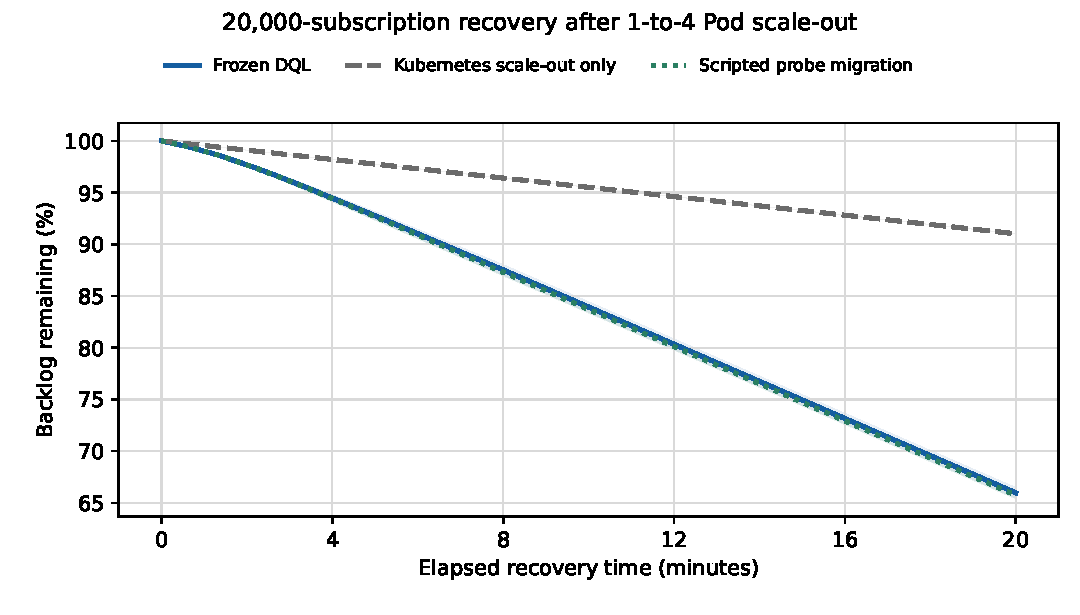
\includegraphics[width=\textwidth]{evidence/persistent-scaleout-recovery-complete/persistent_scaleout_backlog_recovery.pdf}
 \caption{Backlog recovery after adding three subscriber pods. All policies
 start with the same 775-million-event backlog. Curves are means over 20
 paired seeds; shaded bands are descriptive 95\% normal-approximation
 intervals. The area under each normalized curve defines the primary endpoint.}
 \Description{A line chart compares remaining backlog over twenty minutes.
 DQL and scripted probe migration drain substantially more backlog than
 Kubernetes scale-out with the original TCP connection placement.}
 \label{fig:scaleout-backlog-recovery}
\end{figure}

Figure~\ref{fig:scaleout-backlog-recovery} connects the endpoint to the
recovery process. The steeper DQL curve follows successful probe promotions
that place delivery work on additional pods. The nearby scripted-control curve shows that DQL reaches about the same
service capacity as guarded scripted migration. Both improve on the unchanged
placement, establishing the benefit of migration in this workload rather than
a ranking above every controller with the same actions.

\begin{figure}[!htbp]
 \centering
 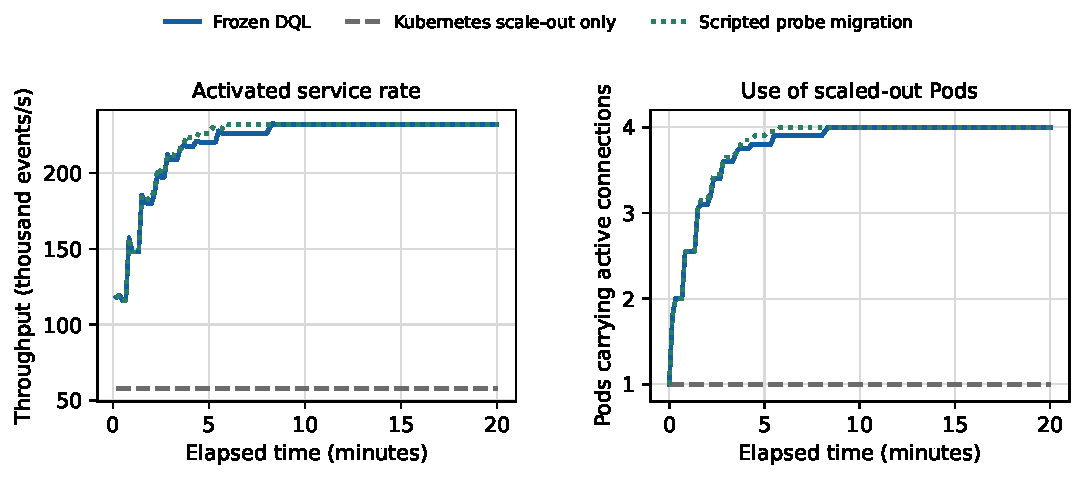
\includegraphics[width=\textwidth]{evidence/persistent-scaleout-recovery-complete/persistent_scaleout_capacity_activation.pdf}
 \caption{Use of the added subscriber capacity. Left: mean delivered events
 per second over each measured interval. Right: mean number of pods carrying
 active client connections. The ten delivery connections are retained as a
 bounded pool while probe promotion replaces their endpoint assignments.}
 \Description{Two line charts show throughput rising as DQL spreads active
 connections across four subscriber pods. The scale-out-only baseline remains
 at one active pod and approximately fifty-eight thousand events per second.}
 \label{fig:scaleout-capacity-activation}
\end{figure}

Figure~\ref{fig:scaleout-capacity-activation} provides the mechanism evidence:
the throughput increase occurs as more pods acquire subscription-bearing
connections. Added pod capacity and client-directed reassociation jointly
produce the gain. In the model's saturated regime, a single pod supplies
approximately 58,000 events/s; four utilized pods supply approximately
232,000 events/s. The mean over the full recovery period is lower because probe discovery
and cooldown take up part of the observation window. The maximum relative difference in queue accounting is $1.45\times10^{-13}$ across the
60 episodes. The simulator represents reassociation as a discrete action;
network delays and the live receipt protocol are outside this timing model.

Figure~\ref{fig:scaleout-violin-distributions} makes the seed-to-seed
variation behind the recovery averages visible. Each AUC observation is the
episode-level quantity in Eq.~\eqref{eq:scaleout-backlog-auc}; each throughput
observation is the episode's delivered-event total divided by its 1,200-second
duration. The violin uses a Gaussian kernel with Scott's bandwidth,
$h=s_{\mathrm{sample}} n_{\mathrm{ep}}^{-1/5}$ for sample standard deviation $s_{\mathrm{sample}}$ and $n_{\mathrm{ep}}=20$, and is drawn only
between the smallest and largest observations. Its width is descriptive, not
a confidence interval. The scale-out-only outcomes are constant because that
policy never changes its initial placement. The adaptive distributions reflect
variation in probe discovery and migration timing. Their separation from the baseline agrees with the paired AUC result above.
The overlapping DQL and scripted distributions describe similar recovery
performance for these two policies, without establishing DQL superiority over
the guarded scripted control.

\begin{figure}[!htbp]
 \centering
 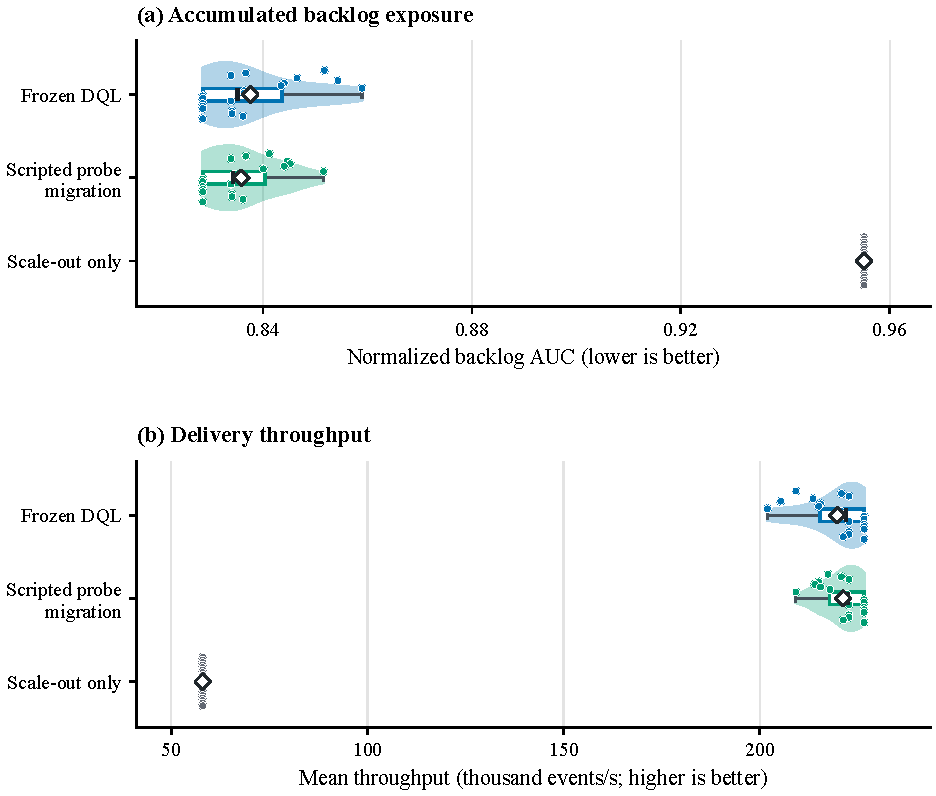
\includegraphics[width=\textwidth]{figures/scaleout-violin-distributions.pdf}
 \caption{Scale-out recovery distributions over 20 paired seeds per policy.
 Violin width shows a kernel-density estimate within the observed range;
 boxes show quartiles and medians, diamonds show means, and points show all
 episodes. Whiskers use the 1.5-interquartile-range rule. The constant
 scale-out-only baseline is shown without an artificial density. Lower
 normalized backlog AUC and higher throughput are preferred.}
 \Description{Two horizontal violin-and-box panels show normalized backlog
 AUC and mean throughput. Frozen DQL and scripted probe migration have lower
 backlog exposure and higher throughput than scale-out alone. Every seed is
 visible; the unchanged-placement baseline has identical values across seeds.}
 \label{fig:scaleout-violin-distributions}
\end{figure}

\paragraph{Independent ad-hoc migration.}
An exploratory extension retains all sixty original observations and adds
eighty episodes: four pressure-unaware schedules evaluated on the same twenty
paired seeds. Each attempt chooses a connection and target Pod uniformly,
without consulting backlog, pressure, or the learned policy. A same-Pod draw
remains a no-op. The schedules use fixed periods of 40 or 60 seconds, or a
60-second nominal period with $\pm30\%$ or $\pm40\%$ uniform timing jitter.
All schedules first act at interval zero. The nominal jitter ranges are
42--78 and 36--84 seconds; rounding upward to the ten-second decision clock
gives executable ranges of 50--80 and 40--90 seconds, respectively. These
percentages modify the schedule, not the measured throughput. Rounding also
changes the average attempt frequency, so jitter is not isolated from timing.
In the following comparison, \emph{Scripted} denotes the independent
60-second schedule with $\pm30\%$ timing jitter; \emph{guarded-greedy migration}
denotes the original pressure-aware positive control. These are distinct
non-learning policies.

\begin{table}[!htbp]
\centering\small
\caption{Independent ad-hoc migration sensitivity in the scale-out simulator. Means over twenty paired seeds per policy; timing jitter changes the schedule, not measured values.}
\label{tab:adhoc-migration}
\begin{tabular}{lrrrr}
\toprule
Policy & Events/s & Backlog AUC & Migrations & Final Pods \\
\midrule
Frozen DQL & 219,762 & 0.83759 & 7.75 & 4.00 \\
Guarded-greedy migration & 221,260 & 0.83589 & 7.75 & 4.00 \\
Ad-hoc: fixed 40 s & 205,295 & 0.84997 & 22.85 & 3.70 \\
Ad-hoc: fixed 60 s & 197,636 & 0.85906 & 15.40 & 3.90 \\
Scripted & 195,737 & 0.86064 & 14.70 & 3.85 \\
Ad-hoc: 60 s, $\pm$40\% & 195,640 & 0.86053 & 14.65 & 3.85 \\
Scale-out only & 58,000 & 0.95510 & 0.00 & 1.00 \\
\bottomrule
\end{tabular}
\end{table}


Table~\ref{tab:adhoc-migration} shows mean DQL throughput of 219,762 events/s,
compared with 195,737 for the $\pm30\%$ schedule and 195,640 for the $\pm40\%$
schedule. The relative gains are 12.27\% and 12.33\%, with pointwise paired
95\% bootstrap intervals of [9.38\%, 15.55\%] and [9.31\%, 15.81\%],
respectively. Each interval uses 10,000 resamples of complete seed pairs and
the ratio of resampled mean rates. DQL uses 7.75 migrations per episode,
compared with 14.70 and 14.65 for the two jittered schedules. The fixed
40-second and 60-second schedules yield gains of 7.05\% and 11.20\%, so the
comparison covers both fixed and jittered schedules. This exploratory
sensitivity analysis reuses the scenario seeds. Its scope is simulated
migration scheduling, separate from independent holdout testing and live
connection-TTL measurements.

\begin{figure}[!htbp]
 \centering
 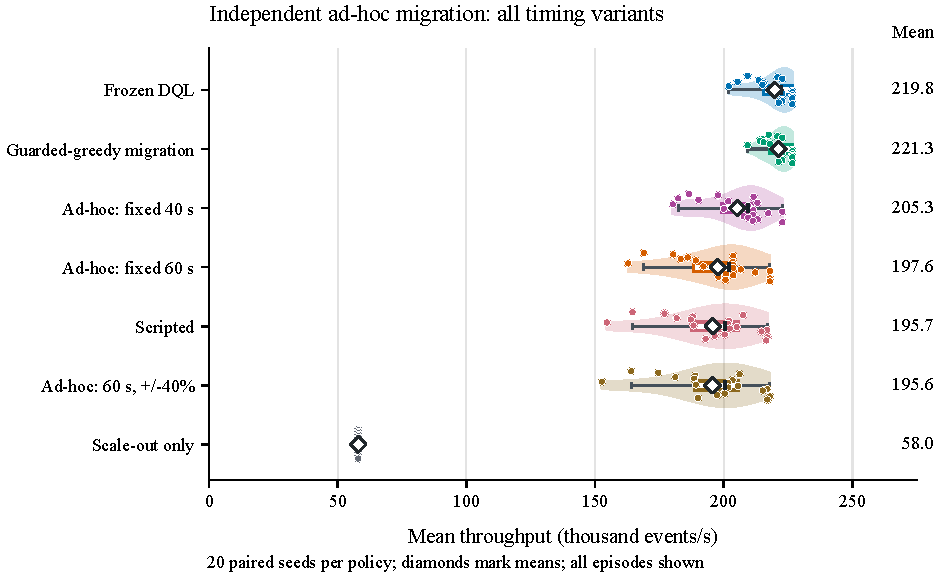
\includegraphics[width=\textwidth]{figures/adhoc-migration-distributions.pdf}
 \caption{Throughput under independent ad-hoc migration schedules. All twenty
 episodes per policy are shown. Violin density uses Scott's bandwidth within
 the observed range; boxes show quartiles and medians, whiskers use the
 1.5-interquartile-range rule, and diamonds mark means. The constant
 scale-out-only control has no artificial density. All seven policies are
 retained, including the original guarded-greedy control.}
 \Description{Seven horizontal violin-and-box rows compare measured simulator
 throughput. DQL has higher mean throughput than every random-endpoint schedule;
 the pressure-aware guarded-greedy control remains close to DQL.}
 \label{fig:adhoc-migration-distributions}
\end{figure}

Figure~\ref{fig:adhoc-migration-distributions} shows the variation hidden by
the averages. Random reassignment can revisit an already occupied Pod or move
work away from a useful placement, whereas the guarded DQL controller admits
pressure-improving candidates. The distributions and migration counts compare
the complete controllers, including their admission and endpoint-selection
rules. The nearby guarded-greedy distribution shows that the result compares
complete policies, including their guards, rather than isolating the effect
of learned action selection.

Figure~\ref{fig:stress-throughput-radar} summarizes the same stressed workload,
rather than importing the mixed-workload radar's averages. Its throughput
coordinate divides each episode's mean rate by the four Pods' combined
nominal capacity, $4\times100{,}000=400{,}000$ events/s. The other coordinates
are the fraction of initial backlog removed, the final active-Pod count
divided by four, and $10/(10+M^{\mathrm{ep}})$ for an episode with $M^{\mathrm{ep}}$ migrations. The last
coordinate decreases with intervention count; it is not a handoff-latency
measurement. Each plotted point averages these per-episode coordinates across
all twenty seeds. No observed-best or policy-specific denominator is used.
The $\pm30\%$ ad-hoc schedule appears alongside the original three controls;
all timing variants remain in Table~\ref{tab:adhoc-migration}.

\begin{figure}[!htbp]
 \centering
 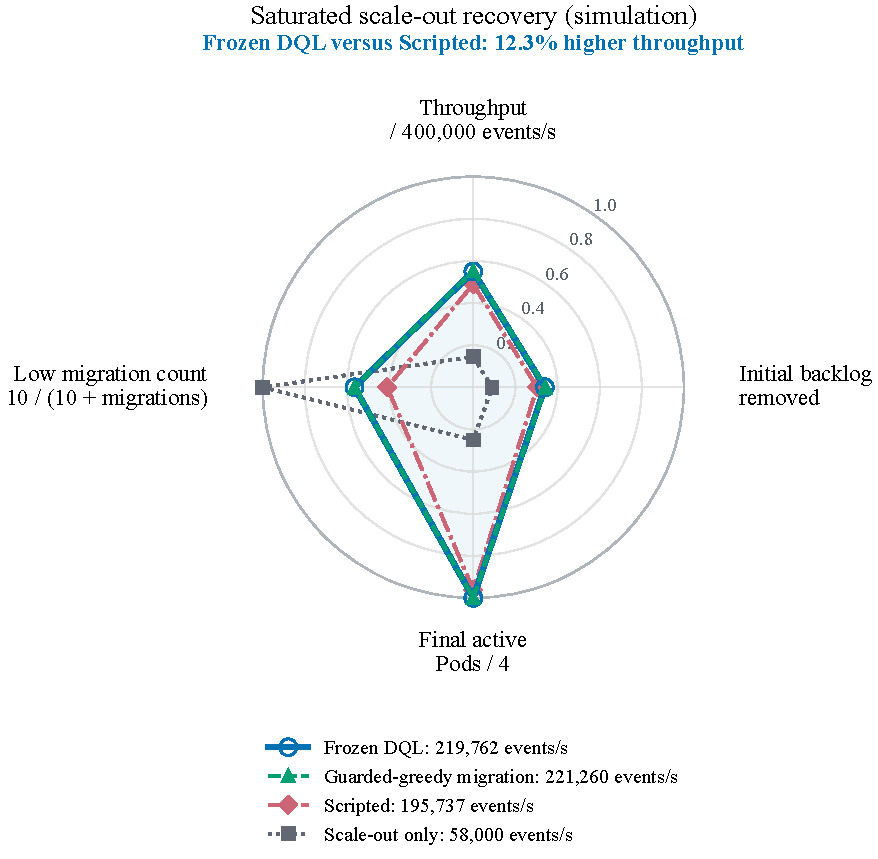
\includegraphics[width=\textwidth]{figures/adhoc-migration-radar.pdf}
 \caption{Stress-scenario radar from all twenty paired simulator seeds per
 displayed policy. \textbf{Frozen DQL versus Scripted: 12.3\% higher throughput},
 with measured mean rates of 219,762 and 195,737 events/s, respectively.
 The guarded-greedy and scale-out-only controls remain visible at 221,260 and
 58,000 events/s. All coordinates use fixed zero-to-one scales, with outward preferred;
 migration count exposes the intervention tradeoff. This is a descriptive
 profile, not an additional objective or statistical test.}
 \Description{A four-axis radar explicitly labels Frozen DQL versus Scripted
 with 12.3 percent higher throughput for DQL.
 It also retains the pressure-aware guarded-greedy and scale-out-only controls,
 and identifies the plotted results as simulator measurements.}
 \label{fig:stress-throughput-radar}
\end{figure}

The DQL throughput radius is 12.3\% larger than the Scripted radius and 3.79 times
the scale-out-only radius because all use the same capacity denominator.
The guarded-greedy comparator has a nearly overlapping profile and slightly
higher mean throughput. The result establishes the benefit of reaching added
capacity, with similar performance from a pressure-aware non-learning control.
Backlog removal and throughput are linked because the workload has no new
arrivals during drainage. They are not independent confirmations. The polygon's
area is not a performance measure. These measurements remain distinct from the Oracle Cloud
expiry and receipt-completion results in Section~\ref{sec:ttl-preload-results}.
\FloatBarrier
